\documentclass[12pt,oneside,a4paper]{article}   
\usepackage[czech, english]{babel}
\usepackage{amsmath}
\usepackage{epsf,epic,eepic,eepicemu,url,graphicx}
\usepackage[utf8]{inputenc}

%% code listings, pretty simple, but works quite ok :-)
\newenvironment{listing}
{\begin{list}{}{\setlength{\leftmargin}{1em}}\item\scriptsize\bfseries}
{\end{list}}

\begin{document}
\begin{center}
\bf MI-VMW 2010/2011\\[2mm]
    \begin{Large}Flickr - feature-based reranking\end{Large}\\[3mm]
       Jiří Mašek (masekji4@fit.cvut.cz)\\
       Jiří Chadima (chadijir@fit.cvut.cz)\\
4.\,12.\,2010
\end{center}

\section{Zadání}
Cílem naší semestrální práce je vytvořit webovou aplikaci, která by našim uživatelům umožňovala vyhledávat obrázky na serveru Flickr \cite{flickr} pomocí klíčových slov a~zároveň podle převažující barvy.

V~práci tedy musíme vyřešit několik úloh: získání výsledku vyhledávání podle klíčových slov ze serveru Flickr.com, extrakce vlastností ze získaných obrázků a~seřazení obrázků podle zadaných parametrů.

Podobnou funkcionalitu nabízí například služba Google Images \cite{GoogleImages}.

\section{Použité technologie}

Rozhodli jsme se použít programovací jazyk Java. Protože nedílnou součástí naší práce je i~webové rozhraní, použijeme variantu Java Enterprise Edition (Java EE). Jako aplikační platformu jsme vybrali volně dostupný, veřejně přístupný a~snadno škálovatelný systém Google App Engine \cite{GoogleAE}, který zdarma poskytuje serverový prostor pro aplikace naprogramované i~v~Java EE.

Pro vývoj jsme použili verzovací systém git, konkrétně veřejně přístupný portál github.com \cite{official}. Pokud je v textu odkazováno k~nějaké vývojové větvi, naleznete ji právě tam.

\section{Získávání obrázků ze serveru Flickr}
Vzhledem k volbě programovacího jazyku bylo pro přístup k API služby Flickr nejjednodušším řešením využití existující knihovny flickrj \cite{flickrj}. Práce s~ní je přitom velice jednoduchá, jak ukazuje následující příklad.

\begin{listing}
\begin{verbatim}
Flickr flickr = new Flickr(API_KEY, SHARED_SECRET, new REST());
SearchParameters sp = new SearchParameters();
sp.setText(keyword);
PhotoList result = flickr.getPhotosInterface().search(sp, perPage, page);
\end{verbatim}
\end{listing}

Výsledkem této sekvence kódu je seznam objektů vyhovujících zadaným parametrům a nacházejících se na dané straně při určeném počtu výsledků na jedné straně.

Tyto objekty v~sobě nesou bližší informace o konkrétní fotografii, kterou reprezentují. Jsou jimi např. identifikátor, rozměry, URL náhledů v~různých velikostech, atd. Objekt taktéž obsahuje metody, které umožňují získat fotografii k~dalšímu zpracování rovnou v~podobě objektu BufferedImage.

V této souvislosti práce rovněž impelentuje jednoduchou cache, která uchovává posledních 50 výsledků hledání, čímž výrazně zrychluje její chod při opakování dotazu se stejným klíčovým slovem.

\section{Hodnocení obrázků}
Pro hodnocení a~řazení obrázků podle referenční barvy se nabízí relativně mnoho postupů a~algoritmů, my jsme se v~naší práci rozhodli zaměřit na rychlost a~zpracování výsledků pokud možno v~reálném čase. Běžnou praxí podobných vyhledávačů je totiž stažení nějakého většího vzorku obrázků, jejich off-line ohodnocení a~posléze uživateli nabízí jen vyhledávání v~této omezené databázi.

Naše implementace se naopak snaží uživateli nabídnout vždy ty poslední fotografie k~daným klíčovým slovům, ačkoliv se některé vypočítané hodnoty ukládají do databáze tak, aby časově náročné výpočty probíhaly pokud možno pro každou fotografii jen jednou.

\subsection{Možnosti porovnávání}
První možností, která se nabízí pro srovnávání barevnosti obrázků s~referenční barvou je metoda popsaná v~\cite{Mueller2k9}. Ta je založená na vytvoření omezené palety barev, na něž se mapuje barva jednotlivých pixelů v~obrázku. Po analýze pixelů tak vznikne histogram této omezené palety, pomocí něhož se dá spočítat vzdálenost různých obrázků vůči referenční barvě, která je rovněž namapována do základní omezené palety barev. Tato metoda se vyznačuje tím, že se výsledná sada obrázků dá velice snadno dále třídit podle dalších barev.

Druhou variantou, která okamžitě vytane na mysl je porovnávání obrázků založené na klasickém RGB histogramu. Jakmile máme spočítaný histogram obrázku, můžeme volit různé metriky pro počítání vzdálenosti od referenční barvy.

\subsection{Extrahované vlastnosti}

V~průběhu implementace jsme zkoušeli subjektivně porovnávat obě metody, a~přišlo nám, že na omezenou sadu obrázků, kterou jsme schopni zpracovat v~pseudo-reálném čase fungují o~něco lépe metody založené na porovnávání RGB histogramů. Co se týče výpočetní a~časové náročnosti, jsou obě metody v~podstatě srovnatelné. Implementace algoritmu vycházejícího z~\cite{Mueller2k9} je dostupná v~repozitáři \cite{official} ve vývojové větvi \textbf{piximilarlike}.

Po získání výsledků vyhledávání ze serveru Flickr tak dochází k~výpočtu histogramu pro každý obrázek pro všechny tři kanály barevného prostoru RGB. Takto získaný histogram je uložen do databáze, kde se uchovává pro budoucí výpočty se stejným obrázkem.

\subsection{Podobnost k referenční barvě}
\label{sec:podobnost}

Pro modelování podobnosti jsme zkoušeli několik metod s~různými úpravami, vždy jsme se však museli držet relativně nízké výpočetní náročnosti kvůli omezení na zpracování v~pseudo-reálném čase.

Nejprve jsme zkoušeli obrázky řadit podle vážené euklidovské vzdálenosti mezi referenční barvou a~nejčastější barvou nacházející se ve spočítaném histogramu (vývojová větev \textbf{peakdistance}). Výsledky takových porovnání nás však příliš neuspokojily a~snažili jsme se nalézt jiné metody.

Nakonec jsme došli k~metodě, která na první pohled nemusí vypadat zcela dokonale, nicméně pro danou aplikaci podává subjektivně poměrně dobré řešení v~rozumném čase. Charakteristické číslo pro každý obrázek, podle kterého budeme obrázky v~této variantě řadit, budeme označovat jako \textbf{váhu obrázku}.

Váha obrázku se vždy skládá ze součtu tří charakteristických čísel vychá-zejících z~histogramů jednotlivých složek RGB modelu. Tato charakteristická čísla jsou počítána podle následujícího algoritmu, kde \texttt{EPSILON} je předem stanovená konstanta, \texttt{baseIndex} je hodnota příslušného kanálu z~referenční barvy a~\texttt{HIST\_SIZE} je šíře histogramu pevně nastavená na 256.

\begin{listing}
\begin{verbatim}
for (int i = baseIndex - EPSILON; i < baseIndex + EPSILON; i++) {
    if (i >= PhotoHistogram.HIST_SIZE) { break; }
    if (i < 0) { continue; }
    sum += histogram.getValue(color, i) *
        (i - baseIndex == 0 ? 1 : Math.abs(i - baseIndex));
    ++values;
}
return (sum / values == 0.0 ? Double.MAX_VALUE : sum / values);
\end{verbatim}
\end{listing}

Algoritmus projde \texttt{EPSILON} okolí referenční barvy a~postupně nasčítá násobky jednotlivých hodnot v~histogramu. Čím dále se pak hodnota nachází od referenční barvy, tím víckrát se do součtu započítává. V případě, kdy by se v daném intervalu \texttt{baseIndex-EPSILON..baseIndex+EPSILON} nacházely samé nulové hodnoty, je takový součet na závěr nahrazen nekonečnem. To zajišťuje, že obrázky, které nemají žádné body alespoň trochu podobné dané barvě, získávají největší váhu a~propadají se řazeným výsledkem dolů. Pos-lední operací je zprůměrování hodnot tak, abychom nemuseli pracovat s~ob-rovskými čísly. Jako nejpodobnější dané barvě je určen obrázek s~\textbf{nejmenší} vahou.

Algoritmus se dá ladit volením hodnoty konstanty \texttt{EPSILON}. Subjektivně nejlepší výsledky algoritmus podává paradoxně při takové hodnotě, kdy se ve smyčce projde celá šířka histogramu.

Zvolený algoritmus má jistě celou řadu menších či větších nedostatků, například není použita žádná metoda normalizace histogramů. To znamená, že obrázky menších rozměrů mají teoretickou výhodu, protože počet jejich pixelů je nižší. Jelikož však načítáme obrázky ze serveru Flickr, které všechny mají stejnou velikost, můžeme tento faktor zřejmě zanedbat.

Na druhou stranu se nám subjektivně zdá, že pro zvolenou aplikaci běžící takřka v~reálném čase je algoritmus poměrně slušně použitelný, ačkoliv docela často dochází k~jasně zřetelným anomáliím.

\subsection{Komentovaná ukázka řazení obrázků}

\begin{figure} \begin{center}
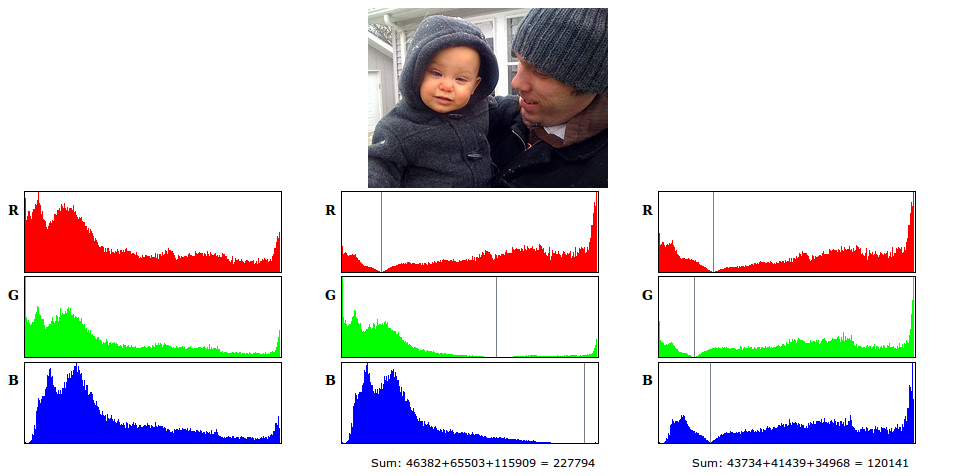
\includegraphics[width=13.5cm]{figs/histogram1.png} \caption{Histogram prvního obrázku}
\label{fig:manchild}
\end{center} \end{figure}
\begin{figure} \begin{center}
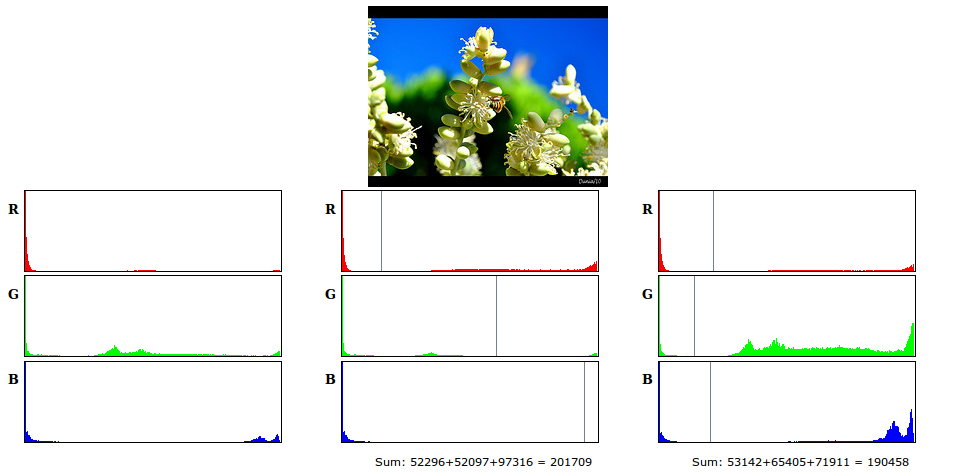
\includegraphics[width=13.5cm]{figs/histogram6.png} \caption{Histogram šestého obrázku}
\label{fig:borderflower}
\end{center} \end{figure}
Pro ilustraci výhod a~nevýhod algoritmu se nyní podívejme na konkrétní příklad řazení.

Celkem řadíme devět obrázků, pro ukázku jsou pro dva konkrétní obrázky uvedeny na obr.~\ref{fig:manchild}~a~ obr.~\ref{fig:borderflower} tři RGB histogramy: normální, ohodnocený pro barvu \verb|#279AF2| a~ohodnocený pro barvu \verb|#362333|. Ohodnoceným histogramem zde rozumíme hodnoty vypočítané pomocí algoritmu uvedeného v~\ref{sec:podobnost}. Šedou čarou je poté vyznačena hodnota kanálu referenční barvy. Pod ohodonocenými histogramy je uvedena i~celková suma těchto hodnot, která vždy slouží jako váha obrázku. Je také nutné čtenáře upozornit, že osy $y$~jednotlivých histogramů mají odlišná měřítka.

\begin{figure} \begin{center}
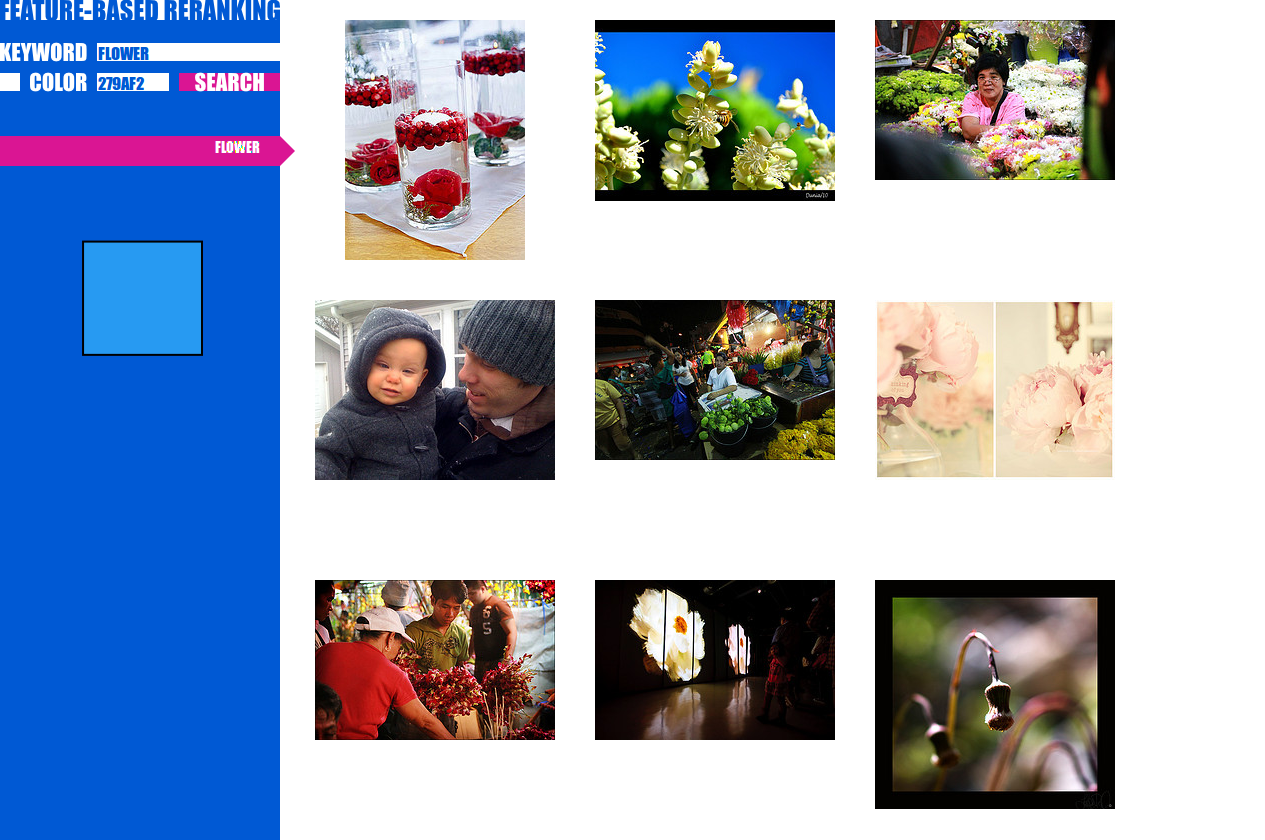
\includegraphics[width=13.5cm]{figs/col01-flower-279af2-withcolor.png} \caption{Obrázky seřazené podle barvy \#279AF2}
\label{fig:279af2}
\end{center} \end{figure}
\begin{figure} \begin{center}
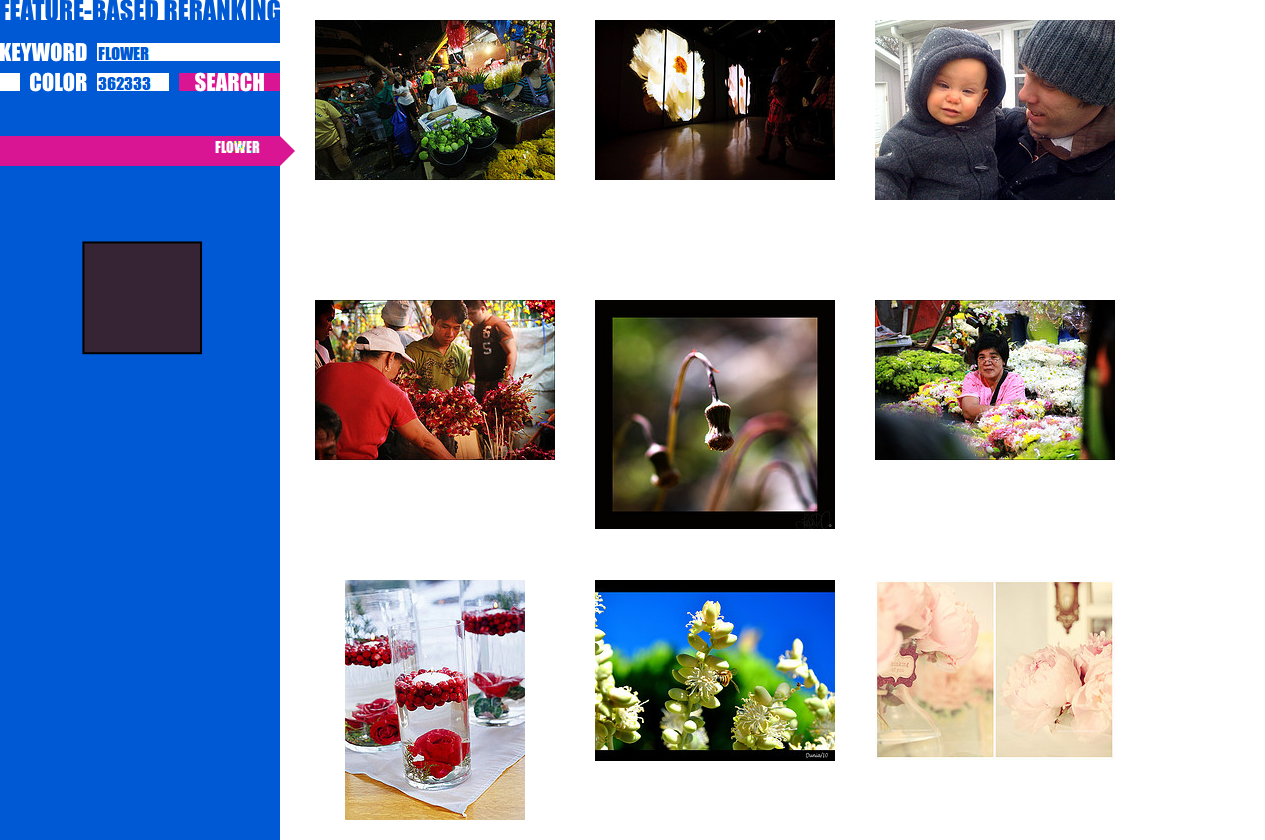
\includegraphics[width=13.5cm]{figs/col01-flower-362333-withcolor.png} \caption{Obrázky seřazené podle barvy \#362333}
\label{fig:362333}
\end{center} \end{figure}

Jak dopadlo výsledné řazení se můžeme podívat na obrázcích \ref{fig:279af2} a~\ref{fig:362333}, kam jsme pro ilustraci doplnili čtverec vyplněný příslušnou barvou, podle které řadíme. Na ukázkových obrázcích \ref{fig:manchild} a~\ref{fig:borderflower} si nyní ukážeme, jak reálně funguje náš algoritmus.

Už u~standardního histogramu je vidět veliký rozdíl v~rozmístění bodů na šíři histogramu. U~obr. \ref{fig:borderflower} vidíme velikou špici u černé barvy, kterou způsobuje černý pruh u~horního a~spodního okraje obrázku. Díky tomu, že v~jednom místě je hodnota výrazně vyšší, než v~těch ostatních, bude algoritmus dobře fungovat v~blízkosti tohoto místa, okolí daného bodu bude započítáno s~nejmenším koeficientem a~vzdálenější místa s~nižšími hodnotami nedají v~součinu tak velká čísla. Oproti tomu při rovnoměrném rozvrstvení hodnot histogramu nebude vzdálenost od referenčního bodu hrát příliš velkou roli.

V~prvním řazení podle barvy \verb|#279AF2| je jako podobnější vyhodnocen obrázek \ref{fig:borderflower}. Je to dáno tím, že do výsledného součtu přispívá většinou malými čísly, jediným velkým číslem je vždy špice u~levého kraje histogramu. Fotografie \ref{fig:manchild} doplácí na to, že jediným ze tří histogramů, kde dochází k~výrazné změně rozložení jednotlivých podílů na výsledném součtu je červený kanál.

U~řazení podle barvy \verb|#362333| se situace obrací. Na obr. \ref{fig:manchild} je krásně vidět, jak se v~modrém a~zeleném histogramu dramaticky změnilo rozdělení jednotlivých podílů na celkovém součtu, kdežto u~obrázku \ref{fig:borderflower} se prakticky nic nezměnilo. Tím, že jsme "trefili" skoro nejčastější barvu v~obrázku \ref{fig:manchild} jsme zajistili její nejnižší podíl na celkovém součtu a~tím v~podstatě i~nejnižší možný celkový součet.

V~součtech u~obrázku \ref{fig:borderflower} si můžeme také všimnout vždy obrovského přís-pěvku modrého kanálu. Opět jde o~efekt jedné velké špice, která (skoro) vždy přispěje velkou měrou do celkového součtu.

Velkou nevýhodou algoritmu je nezávislé posuzování tří kanálů barevného prostoru RGB. Při řazení může dojít k~situaci, kdy nás reálně zajimá řazení pouze podle jednoho kanálu (např. barva \verb|#FF0000|), díky tomu, že vahou je součet součtů všech kanálů nám do řazení zasáhnou i~zbylé dva kanály. Teoreticky zvýhodněny tak budou velmi tmavé obrázky, které obsahují hodně hodnot blízkých nule v~kanálech G~a~B. To může vést k~leckdy zavádějícím výsledkům.

\section{Implementační poznámky}

Google App Engine bohužel neumožňuje použití některých standardních knihoven a~tříd jazyka Java, a~proto jsme museli v~některých částech aplikace sáhnout k~náhradním řešením.

Naše aplikace tak musí obsahovat vlastní implementaci dekodéru formátu JPEG, který jsme převzali z~\cite{Dersch}, protože GAE nepodporuje použití Javovské třídy BufferedImage.

\section{Závěr}

Myslíme si, že v~rámci semestrální práce se nám povedlo implementovat docela použitelný řadící algoritmus, který vyniká poměrně velkou rychlostí, jež je bohužel vykoupena relativně velkou nepřesností algoritmu. Použitá váha obrázku není zcela špatná a~po zapojení některých metod na eliminaci například velkých špicí v~histogramech by se její účinnost mohla ještě zlepšit.

Aplikace je veřejně dostupná na \cite{liveApp}, zdrojové kódy jsou veřejně přístupné k nahlédnutí na \cite{official}.

\renewcommand{\refname}{Literatura}
\bibliographystyle{ieeetr}
{
 \bibliography{refs}
}
\end{document}